\documentclass[11pt,a4paper]{letter}
\usepackage[top=0.50in, bottom=0.5in, left=1.1in, right=1.1in]{geometry}
\usepackage{graphicx}

%\signature{}

\usepackage{Sweave}
\begin{document}

\begin{letter}{}

\includegraphics[width=0.3\textwidth]{logo_uah.png}

\opening{Dear Dr. Wake:}

\noindent Please consider our paper, entitled `Phylogenetic estimates of species-level phenology improve ecological forecasting' as a Letter in \emph{Nature Climate Change}. Our research addresses the critical challenge of accurately predicting the impacts of climate change on plant phenology, with consequences for key ecosystem services, and highlights the importance of incorporating both species variability and phylogenetic information in ecological forecasting.
\vspace{1.5ex}\\
Ecological forecasts often rely on data from a limited number of species, resulting in predictions that fail to capture the high variability observed across species' responses. Hierarchical mixed models (i.e., HMM) have increased their popularity as they can deal with issues related to some species being more data-abundant than others. These models allow inference across species by pooling estimations of data-poor species towards those which are more data rich and implicitly assumes all species are equally interchangeable. However, phylogeny tells us that species are nested within lineages and share a large, but variable, proportion of their evolutionary history with one another. Assumptions of equal exchangeability are thus often invalid.
\vspace{1.5ex}\\
Here, we propose a novel approach that uniquely extends upon the Phylogenetic mixed model (i.e., PMM)   to inform species-level sensitivities to cues. We demonstrate the superior performance of this new formulation compared to commonly used HMMs. We illustrate that species-level variability is greater than variability across cues, emphasizing the importance of accounting for species differences in ecological forecasting. In addition, we show how our approach provides insights into how different clades have evolved phenotypes in response to multiple interacting environmental cues. Our results have important implications for improving ecological forecasting under climate change scenarios with extensions that go beyond the case study of phenology presented here.
\vspace{1.5ex}\\
We believe that our manuscript aligns well with the scope and objectives of \emph{Nature Climate Change}, and we have not submitted it elsewhere. We have suggested three possible reviewers (see online submission system: XX, XX2, XX3). We are grateful for your consideration, and look forward to hearing from you.
\vspace{1.5ex}\\
\noindent Sincerely,\\
\vspace{1.5ex}\\
 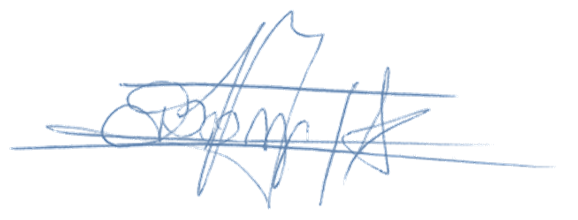
\includegraphics[width=0.2\textwidth]{Signature_IMC.png} \\
 \vspace{1.5ex}\\
\noindent Ignacio Morales-Castilla


\end{letter}
\end{document}
